%
% thc.tex -- Termohaline Zirkulation
%
% (c) 2018 Prof Dr Andreas Müller
%
\chapter{Termohaline Zirkulation\label{chapter:thc}}
\lhead{Termohaline Zirkulation}
\begin{figure}
\centering
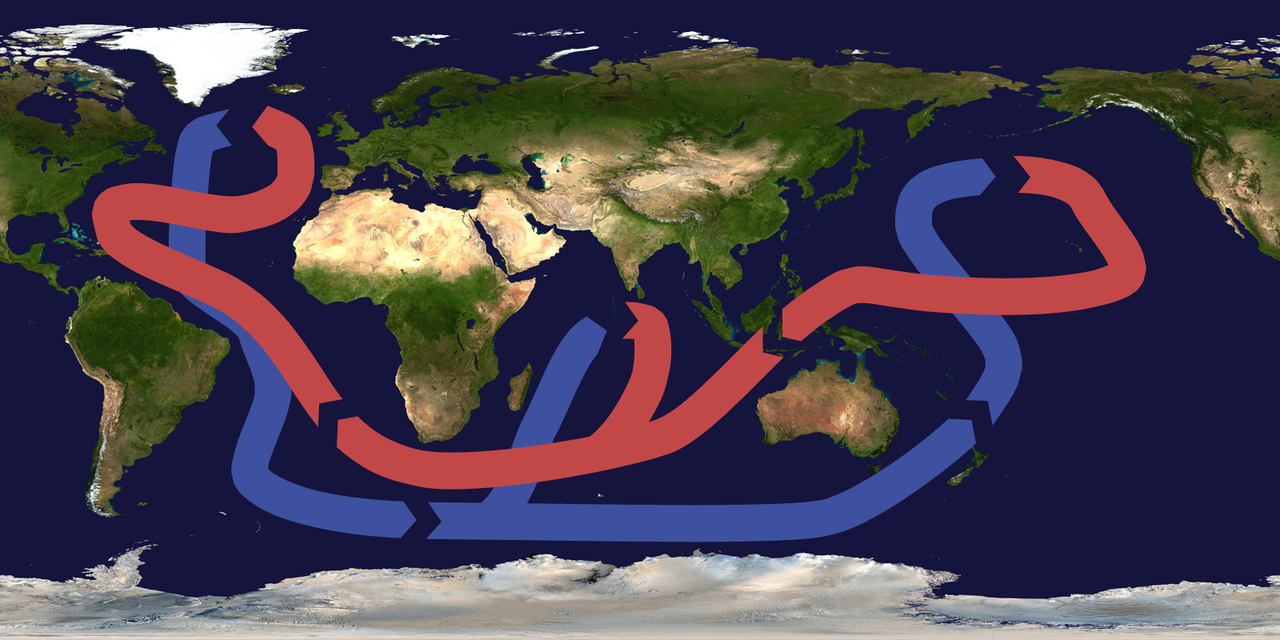
\includegraphics[width=\hsize]{chapters/4/1280px-Thermohaline_circulation.png}
\caption{
Das globale Förderband der thermohalinen Zirkulation.
\label{skript:thc:foerderband}}
\end{figure}%
Der Salzgehalt des Meerwassers ist nicht konstant, beinflusst aber
wie die Temperatur die Dichte.
Dies führt zu einer grossräumigen Zirkulationsströmung in den Weltmeeren,
genannt die thermohaline Zirkulation,
und damit zu einem weiteren bedeutenden Energietransportmechanismus.
Abbildung~\ref{skript:thc:foerderband} zeigt den Umfang der Zirkulation.
Auf einer Zeitskala von Jahrzehnten bis Jahrhunderten wird Meerwasser 
und damit auch Wärmeenergie über Distanzen umgewälzt, welche mehrfach die
Erde umspannen.
Die Organismen, die in den oberen Wasserschichten absterben, sinken langsam
auf den Meeresgrund.
Ohne eine umfassende Umwälzung der Weltmeere würden die oberen Wasserschichten
mit der Zeit an Nährstoffen verarmen.
Die thermohaline Zirkulation stellt also auch die Versorung der
Weltmeere mit Nährstoffen sicher.

Der Golfstrom ist ein kleiner Ausschnitt des globalen Förderbandes.
Die gut bekannte Bedeutung des Golfstroms für das europäische Klima 
deutet an, wie wichtig die thermohaline Zirkulation für das globale
Klima ist.
Es ist daher unerlässlich zu verstehen, was die Zirkulation antreibt und
wie sich der Klimawandel darauf auswirken könnte.

In diesem Kapitel soll die thermohaline Zirkulation modelliert werden.
Besonderes Augenmerk liegt dabei auf der Tatsache, dass dieses System
kippen kann.
Bei einer genügend grossen Änderung der Klimaparameter kann die Zirkulation
sich auf irreversible Art ändern.
Ein solches Ereignis hätte katastrophale Auswirkungen für das Klima.

%
% salinitaet.tex -- Salinität
%
% (c) 2018 Prof Dr Andreas Müller
%
\section{Salinität und Dichte}
\rhead{Salinität}
Der Salzgehalt des Meerwassers ist nicht konstant.
Er steigt an, wenn Wasser verdampf oder sich Eis bildet.
Er sinkt, wenn das Salz durch Niederschläge verdünnt wird.
Mit der Veränderung des Salzgehaltes geht auch eine Änderung
der Dichte einher.


%
% box.tex
%
% (c) 2018 Prof Dr Andreas Müller, Hochschule Rapperswil
%
\section{Ein Modell für die thermohaline Zirkulation}
\rhead{Ein Modell für die thermohaline Zirkulation}
Jedes numerische Modelle der Zirkulation basiert auf einer Diskretisation
des Gebietes.
Der Ozean wird also in kleine Teilgebiete aufgeteilt.
Gesucht sind Temperatur und Salinität in jedem Teilgebiet.
Dann werden Gleichungen aufgestellt, die den Austausch von Salz und
Wärme zwischen den Teilgebieten beschreiben.
Die Lösung dieser Gleichungen wird uns das Ausmass der Zirkulation zeigen
und erlauben abzuschätzen, wie sich die Zirkulation ändert, wenn sich
die äusseren Bedingungen verschieben.

\subsection{Ein einfaches Box-Modell}
Um einen ersten Eindruck von der Dynamik der thermohalinen Zirkulation
zu erhalten, verwenden wir ein Modell mit genau zwei Teilgebieten.
Wir modellieren den Atlantik nördlich des Äquators als zwei Gebiete.
Gebiet 1 ist das Polargebiet mit typischerweise tieferen Temperaturen,
Gebiet 2 ist das Gebiet in der Nähe des Äquators.
In jedem dieser Gebiet modellieren wir nur das Wasser, welches tatsächlich
von der Zirkulation umgewälzt wird.
Wir nehmen an, dass es sich durch die zwei Parameter Temperatur und
Salinität beschreiben lässt.
Wir bezeichnen die Variablen im Gebiet $i$ mit $T_i$ und $S_i$.

Das Wasser, welches an der Zirkulation teilnimmt, ist umgeben von einem
viel grösseren Wasserreservoir, welches mit dem strömenden Wasser 
im Wärme- und Salzaustausch steht.
Wir bezeichnen die konstanten Parameter dieser Reservoirs mit
$T_i^*$ und $S_i^*$.
In Abbildung~\ref{skript:boxmodell-bild} sind die beiden Gebiete
grau dargestellt, das in Zirkulation befindliche Wasser hellblau.
\begin{figure}
\centering
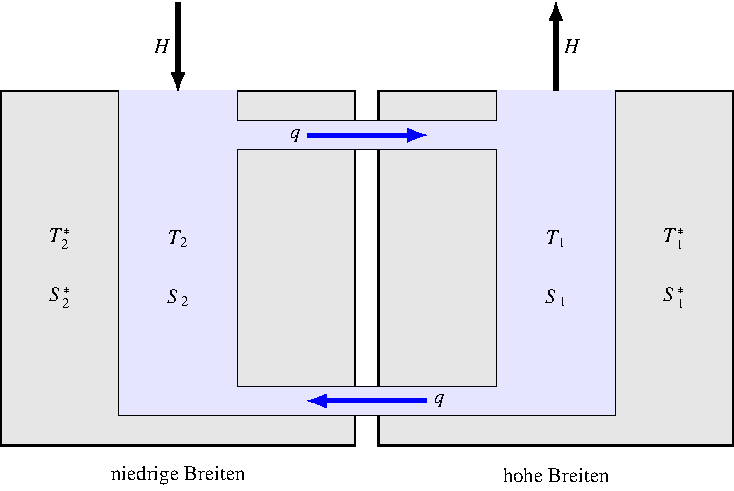
\includegraphics{chapters/4/boxmodell.pdf}
\caption{Einfaches Modell der thermohalinen Zirkulation
\label{skript:boxmodell-bild}}
\end{figure}

Die Zirkulation ist charakterisiert durch den Massefluss $q$ der
Tiefenströmung.
Da kein Wasser verloren gehen kann, muss in Oberflächennähe der gleiche
Fluss herrschen.
Da auch kein Salz verloren gehen kann, müssen sich auch die Salzflüsse
zwischen den beiden Gebieten ausgleichen.
Die Salinität wird zum Beispiel durch die Verdunstung erhöht, während
Niederschlag sie erniedrigt.
Süsswasserflüsse von Kontinenten reduzieren ebenfalls die Salinität.
Dies bedeutet, dass zusätzlich zum Massestrom $q$ ein virtueller 
Salzstrom zwischen den beiden Gebieten herrscht, den wir mit $H$ bezeichnen.

\subsection{Modell-Gleichungen\label{skript:thc:modell-gleichungen}}
Wir müssen jetzt Differentialgleichungen aufstellen, welche die
zeitliche Entwicklung von Temperatur $T_i(t)$ und Salinität $S_i(t)$
beschreiben kann.
Die Temperaturentwicklung wird bestimmt einerseits durch den Energietransport
durch den Fluss $q$ und andererseits durch den Wärmeaustausch mit dem
umgebenden Wasser.
Der Fluss $q$ hat zur Folge, dass sich die Temperaturen $T_1$ und $T_2$
angleichen.
Die beiden Flüsse oben und unten in Abbildung~\ref{skript:boxmodell-bild}
transportieren die gleiche Menge Wasser pro Zeiteinheit.
Es wird also gleichviel Wasser mit Temperatur $T_1$ ins Gebiet $2$ 
transportiert wie Wasser mit Temperatur $T_2$ ins Gebiet $1$.
Das Vorzeichen von $q$ spielt dabei keine Rolle, denn ändert das
Vorzeichen von $q$, fliesst das Wasser mit Temperatur $T_1$ einfach
durch den anderen Kanal.
Die Temperaturänderung von $T_1$ ist also proportional zu $|q|(T_2-T_1)$,
dies legt auch die Masseinheit von $q$ fest.

Der Wärmeaustausch mit dem umgebenden Wasser ist proportional zur
Temperaturdifferenz, wir bezeichnen den Proportionalitätsfaktor mit $c$.
Zusammen mit dem Wärmeaustausch durch die Strömung erhalten wir
die Differentialgleichungen
\begin{equation}
\begin{aligned}
\frac{dT_1}{dt}
&=
c(T_1^*-T_1)
+
|q|(T_2-T_1)
\\
\frac{dT_2}{dt}
&=
c(T_2^*-T_2)
+
|q|(T_1-T_2)
\end{aligned}
\label{skript:thc:temperaturgleichung}
\end{equation}
als Modell für die Temperaturentwicklung.

Analoge Überlegungen müssen wir jetzt auch noch für die Salinität anstellen.
Der Ausgleich der Salinität $S_i$ mit der Salinität $S_i^*$ des
umgebenden Meersbeckens ist proportional zur Differenz, der
Proportionalitätsfaktor, den wir mit $d$ bezeichnen, ist bestimmt durch
die Diffusionsgeschwindigkeit und die turbulente Durchmischung des
zirkulierenden Wassers mit der Umgebung.
Dazu kommt noch der virtuelle Salzfluss $H$:
\begin{equation}
\begin{aligned}
\frac{dS_1}{dt}
&=
\phantom{-}
H
+
d(S_1^*-S_1)
+
|q|(S_2-S_1)
\\
\frac{dS_2}{dt}
&=
-H
+
d(S_2^*-S_2)
+
|q|(S_1-S_2).
\end{aligned}
\label{skript:thc:salinitaetsgleichung}
\end{equation}
Man beachte, dass die Temperaturgleichungen~\eqref{skript:thc:temperaturgleichung}
und die Salinitätsgleichungen~\eqref{skript:thc:salinitaetsgleichung} 
gekoppelt sind, da der Fluss $q$ angetrieben wird vom Dichteunterschied,
der wiederum von Temperatur und Salinität abhängt.

\subsection{Antrieb der Zirkulation}
Die Zirkulation wird vom Dichteunterschied angetrieben.
Es gibt also einen Proportionalitätsfaktor $k$ derart, dass
\[
q = k\frac{\varrho_1 - \varrho_2}{\varrho_0}.
\]
Setzt man die Formel~\eqref{skript:salinity-linear} ein, findet man
\[
q
=
k(-\alpha(T_1-T_2) + \beta(S_1-S_2))
=
k(\alpha(T_2-T_1) + \beta(S_1-S_2))
=
k(\alpha(T_2-T_1) - \beta(S_2-S_1)).
\]
Schreiben wir $\Delta T = T_2-T_1$ und $\Delta S=S_2-S_1$,
dann ist der Fluss nur von den Differenzen abhängig:
\begin{equation}
q=k(\alpha\Delta T-\beta\Delta S).
\label{skript:thc:fluss-delta}
\end{equation}

\subsection{Anomalie-Gleichungen}
Die absoluten Werte von $T_i$ und $S_i$ sind nicht wirklich wichtig,
viel wichtiger sind die Unterschiede $\Delta T_i$ und $\Delta S_i$.
Verschwinden die Differenzen, kommt die Zirkulation zum erliegen,
und dies sind die Phänomene, die wir mit den Gleichungen prognostizieren
können möchten.
Wir streben daher an, die Gleichungen
\eqref{skript:thc:temperaturgleichung}
und
\eqref{skript:thc:salinitaetsgleichung}
in eine Form zu bringen, die nur von Differenzen und Anomalien
abhängt.

Wir schreiben
\[
T_0
=
\frac12(T_1+T_2)
\qquad\text{und}\qquad
S_0
=
\frac12(S_1+S_2)
\]
für die Mittelwerte von Temperatur und Salinität.
Indem wir den Mittelwert der Temperaturgleichungen
\eqref{skript:thc:temperaturgleichung}
bzw.~der Salinitätsgleichung \eqref{skript:thc:salinitaetsgleichung} bilden,
bekommen wir die Gleichungen
\begin{equation}
\begin{aligned}
\frac{dT_0}{dt}
&=
c(T_0^*-T_0)
\\
\frac{dS_0}{dt}
&=
d(S_0^*-S_0),
\end{aligned}
\label{skript:thc:mittelgleichung}
\end{equation}
wobei $T_0^* = \frac12(T_1^*+T_2^*)$ und $S_0^* = \frac12(S_1^*+S_2^*)$.
Die Differentialgleichungen~\eqref{skript:thc:mittelgleichung} 
besagen, dass die mittlere Temperatur des zirkulierenden Wassers
gegen die mittlere Temperatur des umliegenden Meeresbeckens strebt.
Die Faktoren $c$ und $d$ beschreiben, wie schnell der Temperaturausgleich
stattfindet, wie in Abschnitt~\ref{section:zeitkonstanten} ausgeführt wird.

Da die Mitteltemperatur langfristig gegen die Mitteltemperatur der
umliegenden Meeresbecken strebt, liegt es nahe, Temperatur und
Salinität auf diese Mitteltemperatur zu beziehen.
Wir ersetzen also
\begin{equation}
\begin{aligned}
\bar T_1&=T_1-T_0^*,
&
\bar T_2&=T_2-T_0^*
&&\Rightarrow&
\bar T_0&=T_0-T_0^*
\\
\bar S_1&=S_1-S_0^*,
&
\bar S_2&=S_2-S_0^*
&&\Rightarrow&
\bar S_0&=S_0-S_0^*
\end{aligned}
\end{equation}
Die Differentialgleichungen~\eqref{skript:thc:mittelgleichung}
für die Mittelwerte wird damit zu
\begin{align*}
\frac{d\bar T_0}{dt} &= -c \bar T_0\\
\frac{d\bar S_0}{dt} &= -d \bar S_0.
\end{align*}
Die Differentialgleichungen für
$T_i=\bar T_i + T_0^*$
und
$S_i=\bar S_i + S_0^*$
sind
\begin{align*}
\frac{dT_i}{dt}
&=
\frac{d\bar T_i}{dt}
=
c(T_i^*-T_i)
+ |q|\Delta \bar T
=
c(T_i^*- \bar T_i - T_0^*)
+ |q|\Delta \bar T
\\
\frac{dS_i}{dt}
&=
\frac{d\bar S_i}{dt}
=
\pm H
+
d(S_i^*-S_i)
+ |q|\Delta \bar S
=
\pm H
+
d(S_i^*- \bar S_i - S_0^*)
+ |q|\Delta \bar S
\end{align*}
Die Differenzen $T_i^*-T_0^*$ und $S_i^*-S_0^*$ können wir vereinfacht
als
\begin{align*}
T_1^*-T_0^* 
&=
T_1^* - \frac12(T_2^*-T_1^*)
=
-\frac12(T_2^*-T_1^*)
=
-T^*
\\
T_2^*-T_0^*
&=
T_2^*-\frac12(T_2^*-T_1^*)
=
\frac12(T_2^*-T_1^*)
=
T^*
\end{align*}
schreiben und analog für $S^*=\frac12(S_2^*-S_1^*)$.
Damit werden die Differentialgleichungen zu
\begin{equation}
\begin{aligned}
\frac{d\bar T_1}{dt}
&=
c(-T^*-\bar T_1) + |q| (\bar T_2-\bar T_1)
\\
\frac{d\bar T_2}{dt}
&=
c(T^*-\bar T_2) + |q| (\bar T_1-\bar T_2)
\\
\frac{d\bar S_1}{dt}
&=
-H
+
d(-S^*-\bar S_1) + |q|(\bar S_2 - \bar S_1)
\\
\frac{d\bar S_2}{dt}
&=
\phantom{-}H
+
d(S^*-\bar S_2) + |q|(\bar S_1 - \bar S_2)
\end{aligned}
\label{skript:thc:anomaliegleichungen}
\end{equation}
Man beachte, dass die $T^*$ und $S^*$ konstant sind.

In den Gleichungen~\eqref{skript:thc:anomaliegleichungen} hängt
$q$ von den Temperatur- und Salinitätsdifferenzen ab.
Wegen $\Delta\bar T=\Delta T$ und $\Delta\bar S=\Delta S$ ist nach
\eqref{skript:thc:fluss-delta}
\begin{equation}
q = k(\alpha\Delta\bar T-\beta \Delta\bar S).
\label{skript:thc:fluss-delta-anomalie}
\end{equation}

\subsection{Differenzgleichungen}
Wir können die Anomaliegleichungen \eqref{skript:thc:anomaliegleichungen}
noch etwas weiter umformen und die einzelnen Ano\-malien vollständig durch
die Differenzen ersetzen.
Die Differenzen und Summen der Gleichungen sind
\begin{equation}
\begin{aligned}
\frac{d\Delta\bar T}{dt}
&=
c(2T^*-\Delta\bar T)-2|q|\Delta\bar T
&&\qquad&
\frac{d\bar T_0}{dt}
&=
-c\bar T_0
\\
\frac{d\Delta\bar S}{dt}
&=
2H+d(2S^*-\Delta\bar S) - 2|q|\Delta\bar S
&&\qquad&
\frac{d\bar S_0}{dt}
&=
-d\bar S_0.
\end{aligned}
\label{skript:thc:differenzgleichungen}
\end{equation}
Die Gleichungen rechts drücken aus, dass die mittleren Anomalien
exponentiell gegen $0$ gehen.
Die linken Gleichungen beschreiben die Zeitentwicklung der Differenz
der Anomalien.
Man beachte, dass $q$ ebenfalls von den Anomalie-Differenzen abhängt.

\subsection{Zeitkonstanten\label{section:zeitkonstanten}}
\label{skript:thc:zeitkonstanten}
Der Koeffizienten $c$ beschreibt, wie schnell der Temperaturausgleich
durch Wärmeleitung oder turbulente Durchmischung erfolgt.
Der Koeffizient $d$ beschreibt, wie schnell der Salinitätsausgleich
durch Durchmischung und Diffusion stattfinden kann.
Je grösser diese Koeffizienten, desto schneller erfolgt der Prozess.
In den rechten Gleichungen von \eqref{skript:thc:differenzgleichungen}
ist dies ganz offensichtlich.
Vernachlässigen wir für den Moment den Einfluss der Zirkulation,
was wir durch $k=0$ im Ausdruck für $q$ beschreiben können, dann
sehen wir, dass die Differenzgleichungen beide von der Form
einer linearen inhomogenen Differentialgleichung
\[
\frac{d\Delta X}{dt}
=
X^* -cX
\]
sind, wobei $X^*$ eine Konstante ist.
Die Lösung der Gleichung ist
\[
X(t) = \frac{X^*}{c} + C_0 e^{-ct}
\]
mit einer Konstanten $C_0$, die aus den Anfangsbedingungen zu
bestimmen ist.
Die Terme $T^*$, $S^*$ und $H$ verschieben also nur die Lösung,
die Differenzen $\Delta\bar T$ und $\Delta\bar S$ streben exponentiell
wie $e^{-ct}$ bzw.~$e^{-dt}$ gegen diese Gleichgewichtswerte.

Die Grössen $1/c$ und $1/d$ haben die Dimension einer Zeit, wir nennen
sie die {\em Zeitkonstanten} des Prozesses, den $c$ bzw.~$d$ beschreiben.
\index{Zeitkonstante}
Ist zum Beispiel die Zeitkonstante $1/c$ der Temperatur sehr viel kleiner
als die Zeitkonstanten $1/d$ der Salinität, dann bedeutet dies, dass
sich die Temperaturdifferenzen sehr viel schneller ausgleichen als die
Salinitätsdifferenzen.
Für die langfristige Entwicklung der Zirkulation ist in diesem Fall
die Salinitätsentwicklung ausschlaggebend, die Temperaturfunktionen
können durch Konstanten ersetzt werden.





%
% dimensionslos.tex
%
% (c) 2018 Prof Dr Andreas Müller, Hochschule Rapperswil
%
\section{Dynamik der thermohalinen Zirkulation}
\rhead{Dynamik der thermohalinen Zirkulation}
In diesem Abschnitt wollen wir die
Bewegungsgleichung~\eqref{skript:thc:differenzgleichungen}
etwas vereinfachen mit dem Ziel, einzelne Szenarien durchspielen
zu können.
Eine vertiefte Diskussion solcher Modelle ist in
Kapitel~\ref{chapter:thermohalin} zu finden.

\subsection{Elimination von Prozessen mit kurzer Zeitkonstante}
Die Diskussion in Abschnitt~\ref{skript:thc:zeitkonstanten}
ist es zulässig, Variablen mit sehr kleiner Zeitkonstanten
durch Konstanten zu ersetzen.
Tatsächlich erfolgt der Temperaturausgleich im Wasser sehr viel
schneller als der Salinitätsausgleich.
Wir können daher davon ausgehen, dass die Temperaturgleichungen
die Temperaturanomalien sehr schnell gegen eine Gleichgewichtstemperatur
streben lassen und dass wir für die Lösung der Salinitätsgleichungen
mit dieser konstanten Temperatur arbeiten können.

Wir gehen also davon aus, dass $\Delta\bar T=2T^*$ konstant ist und
reduzieren damit das Gleichungssystem
\eqref{skript:thc:differenzgleichungen}
auf die eine Gleichung
\begin{equation}
\frac{d}{dt}\Delta\bar S
=
2H + d(2S^* -\Delta\bar S) - 2|q|\Delta\bar S
\qquad\text{mit}\qquad
q=k(2\alpha T^* -\beta \Delta\bar S).
\label{skript:thc:salinitaetallein}
\end{equation}
Diese Gleichungen beschreiben also die Salinitätsentwicklung unter
der Annahme, dass der Temperaturausgleich sehr schnell erfolgt.
Dieser Ausgleich kann nicht primär durch Durchmischung erfolgen,
denn dieser Mechanimus würde auch die Salinität mit gleicher
vergleichbarer Geschwindigkeit ausgleichen.
Dies bedeutet, dass der dominante Term in der Temperaturgleichung
der Term mit $c$ ist, nicht der Term mit $q$.

Die Gleichung \eqref{skript:thc:salinitaetallein} kann noch nicht auf
einfache Weise gelöst werden.
Wir vereinfachen wir sie daher weiter indem wir ausnutzen, dass 
der Salinitätsausgleich so viel langsamer ist als der Temperaturausgleich,
dass der Term mit $d$ im Vergleich zum Term mit $q$ vernachlässigbar ist.
Wir setzen also $d=0$ und
erhalten damit 
\begin{equation}
\frac{d}{dt}\Delta\bar S
=
2H - 2|q|\Delta\bar S
\qquad\text{mit}\qquad
q=k(2\alpha T^* -\beta \Delta\bar S)
\label{skript:thc:qgleichung}
\end{equation}
als vereinfachte Differentialgleichung zur Modellierung der 
thermohalinen Zirkulation.
Dies ist eine nichtlineare Differentialgleichung erster Ordnung,
die nicht in geschlossener Form gelöst werden kann.

\subsection{Eine dimensionslose Beschreibung}
Die Gleichung \eqref{skript:thc:qgleichung} ist wegen der vielen
Konstanten unübersichtlich.
Ausgeschrieben lautet sie
\begin{equation}
\frac{d}{dt}\Delta\bar S
=
2H
-2k\,|\alpha\Delta\bar T- \beta \Delta\bar S|\,\Delta\bar S
\label{skript:thc:smitdim}
\end{equation}
Die meisten der Konstanten können wir aber los werden, indem wir 
die unabhängigen Variablen und die Zeit neu skalieren.
Dies ist gleichbedeutend mit einem Wechsel der Masseinheiten.
Wir verwenden:
\begin{equation}
x=\frac{\beta\Delta\bar S}{\alpha\Delta\bar T},
\qquad
\tau = 2\alpha k\,|\Delta\bar T|\, t
\qquad\text{und}\qquad
\lambda = \frac{\beta H}{\alpha^2 k\Delta\bar T|\Delta\bar T|}.
\label{skript:thc:masseinheiten}
\end{equation}
Die Ableitung nach $t$ kann durch die Ableitung nach $\tau$ ausgedrücket
werden vermöge der Ersetzung
\[
\frac{d}{d\tau}
=
\frac{1}{2\alpha k|\Delta\bar T|}
\frac{d}{dt}
\qquad\Rightarrow\qquad
\frac{d}{dt}
=
2\alpha k|\Delta\bar T|\frac{d}{d\tau}.
\]
Setzen wir dies in die Gleichung~\eqref{skript:thc:masseinheiten}
ein, erhalten wir
\begin{equation}
2\alpha k|\Delta\bar T|
\frac{d}{d\tau} \Delta\bar S
=
2H-2k|\alpha\Delta\bar T-\beta\Delta\bar S|\,\Delta\bar S.
\end{equation}
Wir erweitern mit $\beta/\alpha\Delta\bar T$, damit wird die
Differentialgleichung zu
\begin{align}
2\alpha k|\Delta\bar T|
\frac{d}{d\tau}\frac{\beta\Delta\bar S}{\alpha\Delta\bar T}
&=
\frac{2\beta H}{\alpha\Delta\bar T} - 2k|\alpha\Delta\bar T-\beta\Delta\bar S|\,
\frac{\beta\Delta\bar S}{\alpha\Delta\bar T}
\notag
\\
\alpha k|\Delta\bar T|
\frac{d}{d\tau}x
&=
\frac{\beta H}{\alpha\Delta\bar T}
-k|\alpha\Delta\bar T-\beta\Delta\bar S|\, x
\notag
\\
k
\frac{d}{d\tau}x
&=
\frac{\beta H}{\alpha^2\Delta\bar T\,|\Delta\bar T|}
-k\biggl|1-\frac{\beta\Delta\bar S}{\alpha\Delta\bar T}\biggr|\,x
\notag
\\
\frac{d}{d\tau}x
&=
\frac{\beta H}{k\alpha^2\Delta\bar T\,|\Delta\bar T|}
-\biggl|1-\frac{\beta\Delta\bar S}{\alpha\Delta\bar T}\biggr|\,x
\notag
\\
\frac{dx}{d\tau}
&=
\lambda - |1-x|x.
\label{skript:thc:dimensionslos}
\end{align}
Damit haben wir die ursprüngliche Gleichung
\eqref{skript:thc:smitdim}
in eine dimensionslose Gleichung mit dem einen Parameter $\lambda$
umgewandelt.
%Das Verhalten der Lösung hängt vom Parameter $\lambda$ ab.

\subsection{Gleichgewicht}
Um das Verhalten der Lösungen von 
\eqref{skript:thc:dimensionslos}
besser zu verstehen, suchen wir zunächst nach Gleichgewichtslösungen.
Diese hängen nicht von der Zeit ab, es gilt also
\begin{equation}
\frac{dx}{d\tau}=0
\qquad\Rightarrow\qquad
\lambda-|1-x|x=0
\qquad\Rightarrow\qquad
|1-x|x
=
\lambda.
\label{skript:thc:lambdagl}
\end{equation}
\begin{figure}
\centering
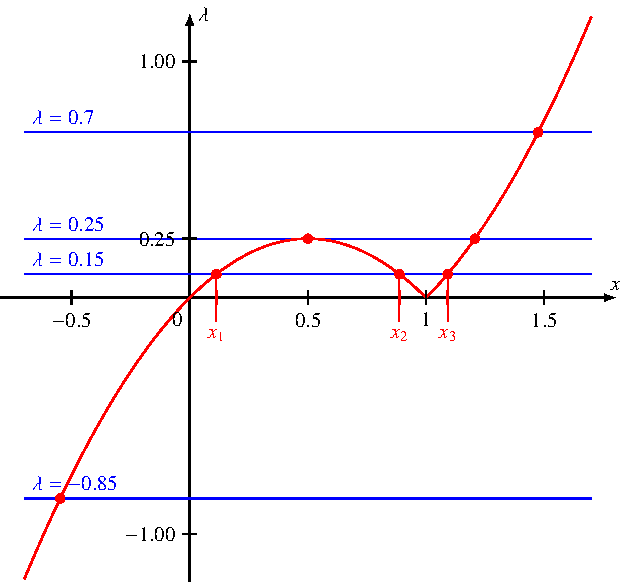
\includegraphics{chapters/4/rhs.pdf}
\caption{Graph der Funktion $|1-x|\,x$ und
Gleichgewichtslösungen der dimensionslosen Differentialgleichung
\eqref{skript:thc:dimensionslos}
\label{skript:thc:1-xxgraph}}
\end{figure}%
In Abbildung~\ref{skript:thc:1-xxgraph} ist der Graph der Funktion 
$|1-x|\,x$ dargestellt.
Je nach dem Wert von $\lambda$ hat die dimensionslose Differentialgleichung
\eqref{skript:thc:dimensionslos} bis zu drei Gleichgewichtslösungen.

Für Werte von $\lambda$ zwischen $0$ und $0.25$ gibt es drei verschiedene
Werte $x$, die die Gleichung \eqref{skript:thc:lambdagl} erfüllen
(Abbildung~\ref{skript:thc:drei}).
Für $x\le 1$  ist $1-x\ge 0$ und damit muss $x$ die 
Gleichung $(1-x)x=\lambda$ erfüllen, für $x\ge 1$ ist es die Gleichung
$(x-1)x=\lambda$.
Diese beiden Gleichungen haben die folgenden Lösungen
\begin{align*}
&\text{Fall $x \le 1$:}
&
(1-x)x&=\lambda
&
&\text{Fall $x\ge 1$:}
&
(x-1)x&=\lambda
\\
&&
x^2-x+\lambda&=0
&&&
x^2-x-\lambda&=0
\\
&&
x&=\frac12\pm\sqrt{\frac14-\lambda}
&&&
x&=\frac12+\sqrt{\frac14+\lambda}.
\end{align*}
Die rechte Gleichung hat für alle Werte $\lambda > 0$ zwar auch noch
eine Lösung $<1$, diese ist aber ausgeschlossen, daher nur das
positive Zeichen vor der Wurzel in diesem Fall.
Für $\lambda > 0.25$ hat die linke Gleichung keine Lösung.
Für $\lambda < 0$ ist die Lösung mit dem positiven Zeichen der linken
Gleichung ausgeschlossen.

\begin{figure}
\centering
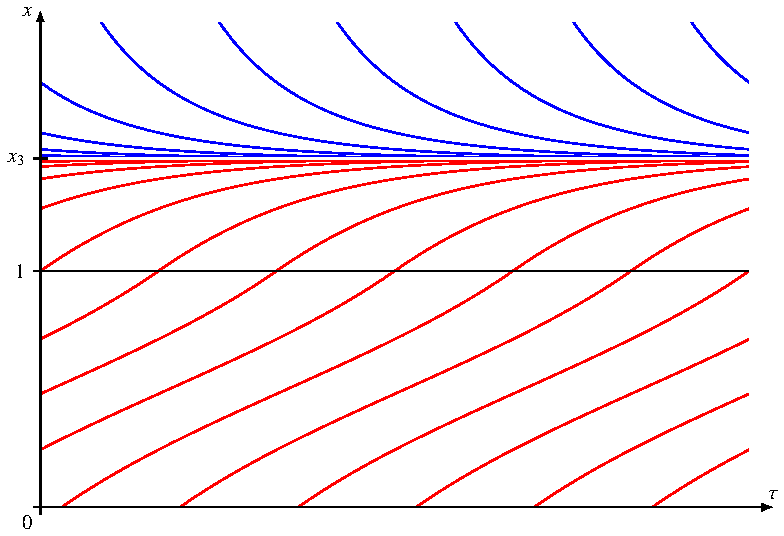
\includegraphics{chapters/4/ein.pdf}
\caption{Lösungen im Fall $\lambda > \frac14$: der einzige
Gleichgewichtspunkt $x_3$ ist stabil.
\label{skript:thc:ein}}
\end{figure}%
Wir berechnen die Lösung der Differentialgleichung für einen gegebenen
Wert von $\lambda$ (Abbildung~\ref{skript:thc:ein}).
Für $\lambda >\frac14$ gibt es nur einen Gleichgewichtspunkt, wir 
nennen ihn $x_3$.
Falls $x(\tau)<x_3$, dann ist
\[
\frac{dx}{d\tau}
=
\lambda - |1-x|x > 0,
\]
die Lösung $x(\tau)$ ist also monoton wachsend.
Für $x(\tau) > x_3$ ist hingegen
\[
\frac{dx}{d\tau}
=
\lambda - |1-x|x < 0,
\]
die Lösung ist also monoton fallend.
Lösungskurven, die bei $x$-Werten $>x_3$ beginnen nehmen monoton ab
und konvergieren gegen $x_3$, solche, die bei $x$-Werten $<x_3$ beginnen,
nehmen monoton zu und konvergieren von unten gegen $x_3$.
Die Gleichgewichtslösung $x(\tau)=x_3$ ist also eine stabile Lösung,
alle anderen Lösungen konvergieren gegen diese Lösung.

\begin{figure}
\centering
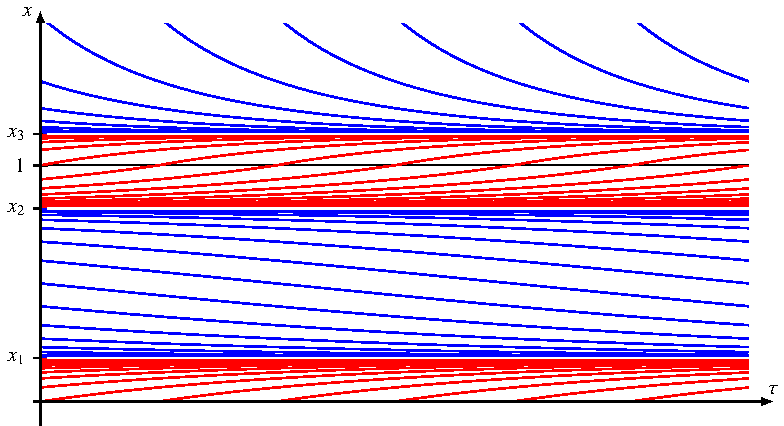
\includegraphics{chapters/4/drei.pdf}
\caption{Lösungen im Fall $0\le \lambda\le\frac14$: die beiden
Gleichgewichtspunkte $x_1$ und $x_3$ sind stabil, $x_2$ ist instabil.
\label{skript:thc:drei}}
\end{figure}%
Für $0<\lambda<\frac14$ seien
$x_1$, $x_2$ und $x_3$ die drei Gleichgewichtspunkte
(Abbildung~\ref{skript:thc:drei}).
Wir untersuchen wieder die Vorzeichen von $dx/d\tau$. 
Für $x$-Werten zwischen $x_1$ und $x_2$ und für $x$-Werte grösser
als $x_3$ ist die Ableitung positiv, die Lösungen konvergieren monoton
wachsend gegen die Gleichgewichtslösungen $x_1$ bzw.~$x_3$.
Lösungen, die bei $x<x_1$ oder $x_2<x<x_3$ beginnen, konvergieren
dagegen monoton wachsend gegen $x_1$ bzw.~$x_3$.
Die Gleichgewichtslösung $x_2$ ist daher nicht stabil,
die Gleichgewichtslösungen $x_1$ und $x_3$ sind dagegen stabil.

\subsection{Bifurkation}
In diesem Abschnitt studieren wir die Abhängigkeit der Gleichgewichtslösungen
in Abhängigkeit vom Parameter $\lambda$, wie dies in Abschnitt
\ref{section:bifurkation-eindim} vorbereitet wurde.

\begin{figure}
\centering
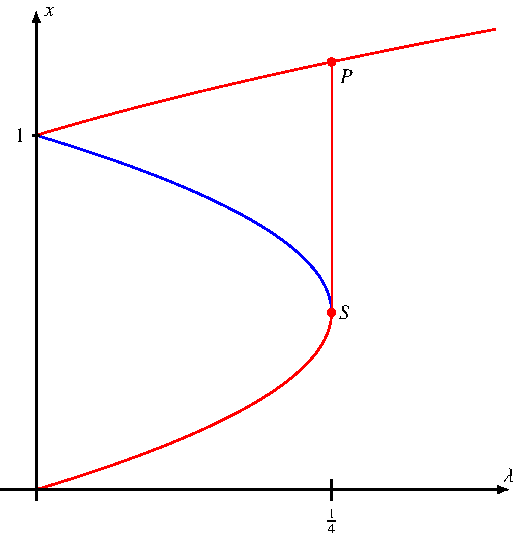
\includegraphics{chapters/4/bi.pdf}
\caption{Bifurkationsdiagramm für die Differentialgleichung
\eqref{skript:thc:lambdagl}
\label{skript:thc:bifurkation}}
\end{figure}
Für Parameterwerte $\lambda < \frac14$ gibt es drei mögliche
Gleichgewichtspunkte, für $\lambda>\frac14$ jedoch nur noch einen.
Wir möchten untersuchen, wie sich die Lösung verhält, wenn der
Parameter langsam verändert wird.
Dies ist in Abbildung~\ref{skript:thc:bifurkation} dargestellt.

Sei jetzt also zunächst $\lambda <\frac14$.
Wir betrachten eine Lösung, die in Nähe von
\[
x_1(\lambda)=\frac12-\sqrt{\frac14-\lambda}
\]
beginnt.
Vergrössern wir $\lambda$, verschiebt sich der Gleichgewichtspunkt
$x_1(\lambda)$ ebenfalls nach oben.
Da $x_1(\lambda)$ aber ein stabiler Gleichgewichtspunkt ist, wird die
Lösung gegen den neuen Gleichgewichtspunkt konvergieren.
Das gleiche passiert auch, wenn die Lösung in der Nähe von
\[
x_3(\lambda)=\frac12+\sqrt{\frac14+\lambda}
\]
beginnt.
Bei einer Vergrösserung folgt das System den roten Kurven in
Abbildung~\ref{skript:thc:bifurkation}.

Wenn jetzt aber der Parameter $\lambda$ die Schwelle $\frac14$
überschreitet, dann wird die Lösung zum einzigen verbleibenden
stabilen Gleichgewichtspunkt $x_3(\lambda)$ konvergieren.
Die Lösung springt also vom Punkt $S$ zum Punkt $P$ auf dem oberen roten Ast
in Abbildung~\ref{skript:thc:bifurkation}.

Wenn man den Parameter $\lambda$ wieder verkleinert, dann wird
eine Lösung in der Nähe von $x_3(\lambda)$ wieder gegen
$x_3(\lambda)$ konvergieren.
Es ist aber nicht mehr möglich, dass die Lösung gegen $x_1(\lambda)$
konvergiert, da nach Abbildung~\ref{skript:thc:drei} nur Lösungen,
die bei $x$-Werten $<x_2$ beginnen, gegen $x_1(\lambda)$ konvergieren
können.

Dieses einfache Modell der thermohalinen Zirkulation hat also die
überraschende Eigenschaft, dass das System beim Überschreiten des
kritischen Wertes $\lambda=\frac14$ in einen Zustand kippt, aus dem
es nicht mehr zurück kommen kann.
Wegen
\[
\lambda
=
\frac{\beta H}{\alpha^2k\Delta\bar T\,|\Delta\bar T|}
\]
kann dies passieren wenn entweder der Betrag des virtuellen Salzflusses 
$H$ ansteigt oder die Temperaturanomaliedifferenz $\Delta\bar T$
klein wird.
Eine Klimaerwärmung könnte zum Beispiel die Verdunstung im Gebiet $2$
erhöhen, den virtuellen Salzfluss erhöhen und damit das System
in den Zustand mit einer wesentlich grösseren Anomaliedifferenz
$\Delta\bar S$ kippen lassen.









